%!TEX root = these.tex

\chapter[Exploitation de VFA pour l'aide à la sélection]{Exploitation du modèle VFA pour la conception de technique de sélection}
\minitoc
\label{chap5}
\cleardoublepage

\section{Introduction}
	Dans ce chapitre, nous présentons premièrement différentes pistes pour concevoir des techniques d'aide à la sélection (ou améliorer des techniques existantes) à l'aide de l'ensemble des enseignements tirés des précédents chapitres, et en particulier du modèle VFA et de son pouvoir de prédiction de la difficulté de sélection d'une cible mobile.
	Deuxièmement, nous exposons un protocole expérimental permettant de valider ce type d'exploitation du modèle VFA, puis nous présentons et analysons les résultats de l'étude empirique menée selon ce protocole.
	Troisièmement, nous proposons une nouvelle technique de sélection, dont la conception s'appuie sur les travaux présentés plus haut dans ce manuscrit.
	Enfin, nous portons un regard critique sur nos résultats, et détaillons une réflexion sur les travaux futurs à mener.
	
\section[VFA : guide pour la sélection de cibles mobiles]{Le modèle VFA comme guide pour les tâches de sélection de cibles mobiles}
	Les résultats que nous avons obtenus et exposés au cours du chapitre~\ref{chap4} montrent, comme de nombreux travaux antérieurs, que la vitesse a un effet déterminant sur les performances de sélection. La première recommandation qui découle de cette observation est de chercher à réduire la vitesse réelle ou effective des cibles mobiles pour en faciliter la sélection.

	Mais comme nous l'avions vu dans le chapitre~\ref{chap4}, la pseudo-entropie, c'est-à-dire le produit AF, a également une influence importante sur les performances de sélection à une vitesse donnée, et permet dans une certaine mesure de les prédire. C'est ce qu'illustre la figure~\ref{fig:tAF} de la section~\ref{sub:previsibility}. Or, l'étude menée sur les périmètres et aires des enveloppes convexes des trajectoires, telle que présentée dans le même chapitre, suggère une plus grande pertinence de la valeur $A\sqrt{F}$, que nous appellerons dorénavant pseudo-entropie subjective, ou PES. Aussi nous apparaît-il judicieux de revisiter la relation entre les performances de sélection et les paramètres VFA, que nous illustrons par la figure~\ref{fig:tAsqrtF}.
	
	\begin{figure}[!htb]
		\centering
		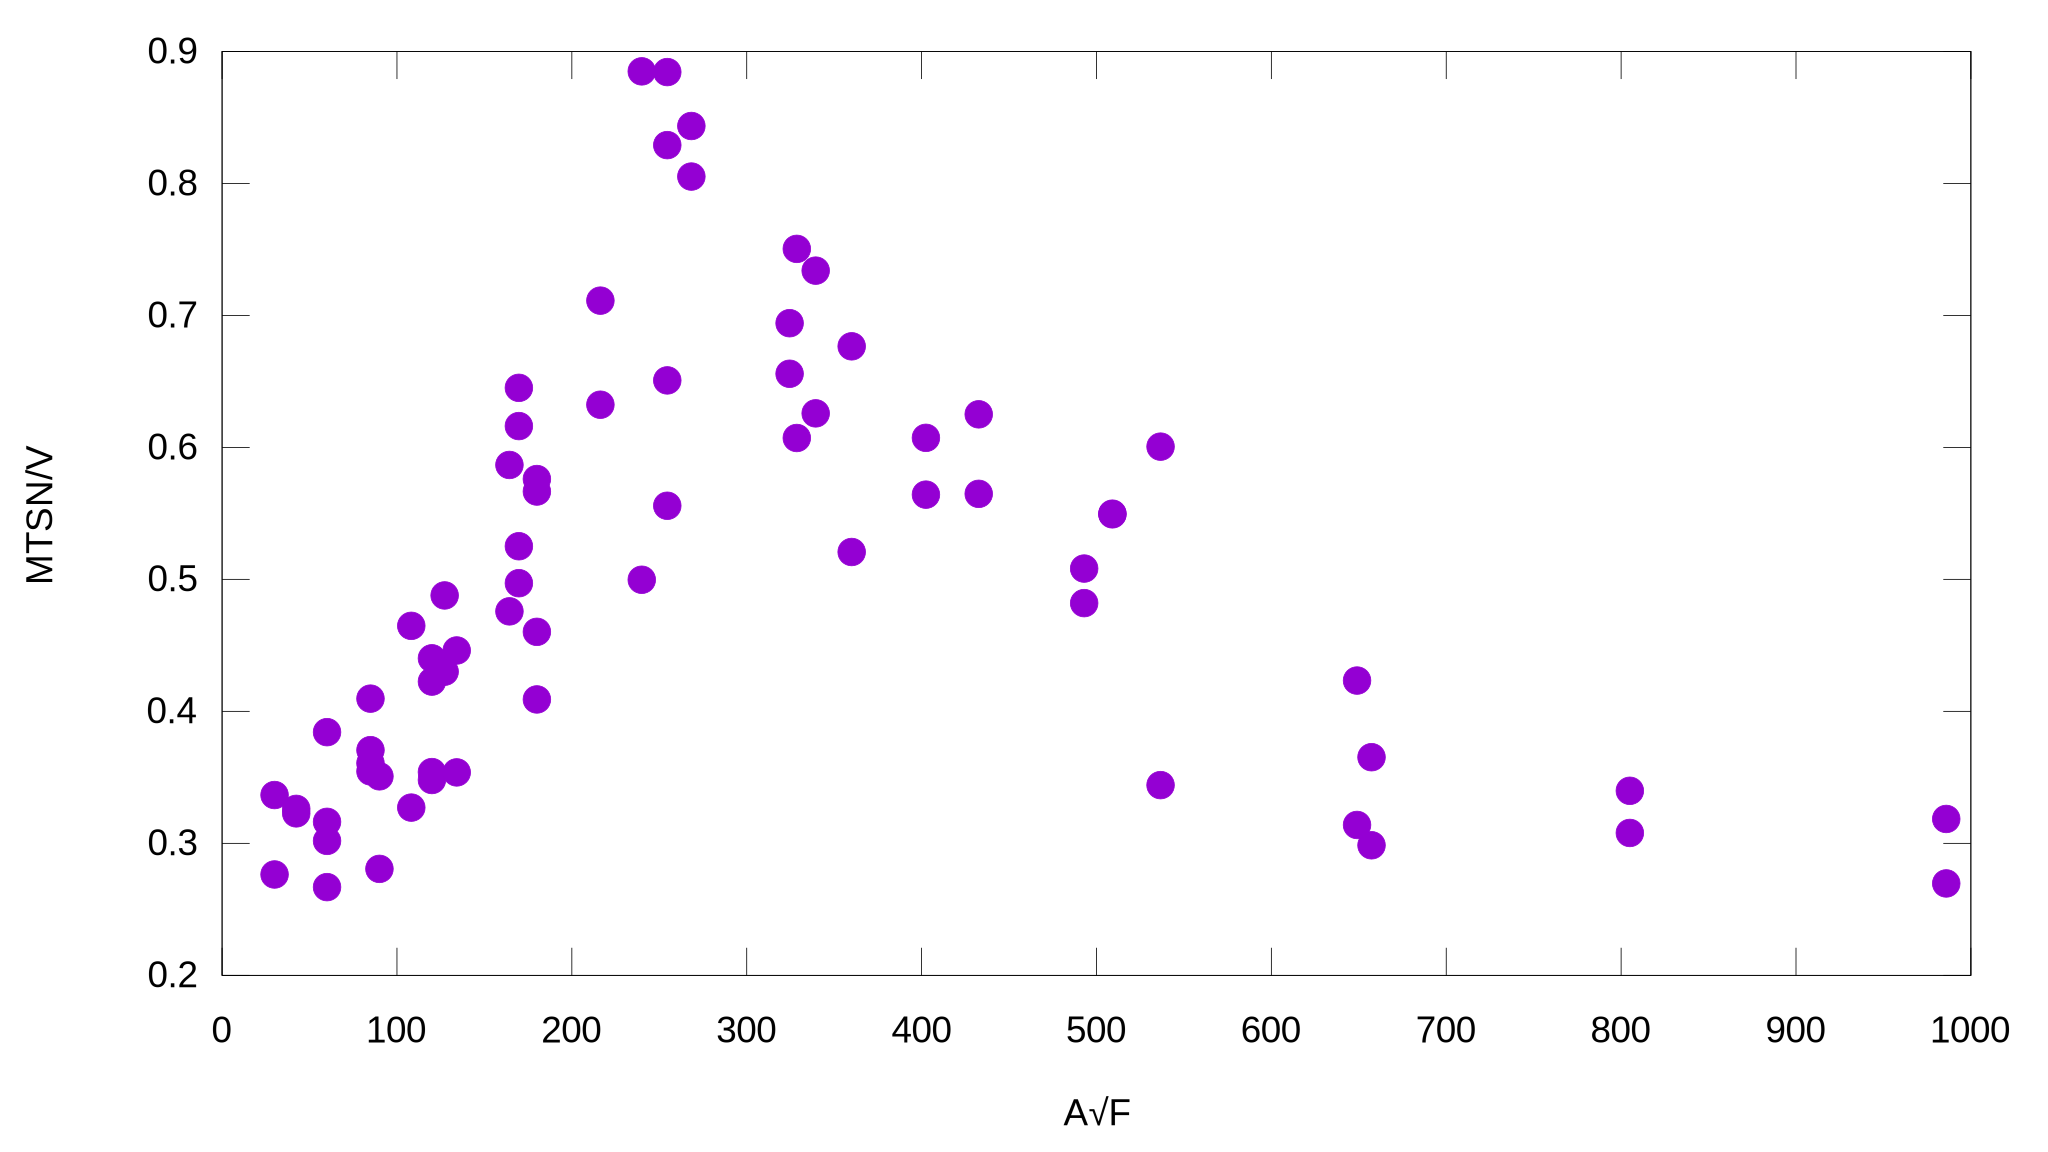
\includegraphics[width=0.8\textwidth]{figures/ch5/asqrtFvTime}
		\caption{Moyennes des temps de sélection normalisés, divisées par la vitesse, en fonction du produit $A\sqrt{F}$, pour des cibles de vitesse moyenne ou rapide.}
		\label{fig:tAsqrtF}
	\end{figure}
	
	Celle-ci nous apprend que lorque la valeur de $A\sqrt{F}$ est autour de 250~$\degree{}Hz^{\frac{1}{2}}$, les temps de sélection sont maximaux. Nous appellerons cette valeur $PES_{max}$. De manière analogue, il est possible de considérer le produit AF, auquel cas cette valeur se trouve autour de 1200~\textdegree{}Hz. Compte tenu des résultats du chapitre 4, il est préférable d'utiliser le produit $A\sqrt{F}$.
	
	Nous pouvons donc en tirer une recommandation pratique simple : chercher à s'éloigner de ces valeurs de référence. Ainsi, la conception d'une application impliquant la sélection de cibles mobiles devrait inclure une phase d'estimation de la pseudo-entropie ou, de manière équivalente et peut-être plus pertinente, de $A\sqrt{F}$. Puis, une phase de réflexion sur les manières dont il serait possible de modifier le comportement des cibles pour s'éloigner de la valeur correspondant à la difficulté maximale.
	
	Concrètement, si la valeur de $A\sqrt{F}$ estimée est inférieure à 250, il faudra chercher à diminuer A ou F ; si elle est supérieure, il faudra chercher à les augmenter. Dans un contexte vidéoludique, par exemple, cela implique de modifier les paramètres de mouvement des objets, si cela n'a pas d'effet délétère sur les mécanismes de jeu. Dans d'autres contextes applicatifs, il n'est pas forcément aisé de modifier le comportement intrinsèque des objets.
	
	Toutefois, cette recommandation pratique vaut autant pour la conception d'applications que pour l'élaboration de techniques d'aide à la sélection. En effet, certaines des techniques de sélection étudiées dans le chapitre~\ref{chap2} sont fondées sur la modification de la taille effective des cibles ou de leur distance au curseur ; lorsqu'il s'agit de cibles mobiles, elles peuvent également agir sur la vitesse, dont nous savons que l'importance est primordiale.
	
	Dans la plupart des contextes applicatifs que nous avons étudiés, la PES d'une cible est généralement en dessous de $PES_{max}$. Pour l'en éloingner encore plus, il faut donc chercher à diminuer A et F.
	
	\subsection{Méthodes pour la modification du paramètre F}

	
\clearpage